\chapter{گزارش پایان  نامه کنترل آرایش مجموعه ای از رباتهای همکار جهت جابجایی جسم}

\section{فصل 1
\\
مقدمه و بیان مسئله}
\subsection{چکیده:}
در این پایان نامه سه نوع روش برای انجام پروژه در نظر گرفته شده است.
1- کنترل آرایش جهت هماهنگی میان رباتها برای حمل بار با استفاده از روش رهبر - پیرو در طراحی این روش کنترل آرایش، با توجه به مسیر جسم، مسیر مطلوب برای رهبر گروه مشخص می‌شود.
\\
2- طراحی کنترل آرایش بر مبنای روش ساختار مجازی. در این استراتژی علاوه بر تعقیب مسیرهای مطلوب رباتها روش 
\lr{mutual feedback}
جهت مقاوم سازی گروه در مقابل اغتشاشات وارده بر رباتها جهت حفظ آرایش در نظر گرفته شده است.
\\
3- با ترکیب میدان پتانسیل با بازخورد آرایش روش مناسبی جهت عبور مجموعه رباتها از میان موانع و رسیدن به هدف مورد نظر است.
\\
4- برای حمل جسم الگوریتم کنترل امپدانس چندگانه به عنوان روش کنترل موثر جهت تعقیب مسیرهای مطلوب بر روی ربات‌های همکار به همراه جسم مورد جابجایی با روش ساختار مجازی اعمال می‌شود.
\\
5- آرایشش بهینه‌ی گروه جهت حمل بار در مسیرهای مشخص به وسیله الگوریتمهای بهینه سازی بدست آمده است.

\subsection{مقدمه و بیان مسئله:}
در ابتدا یک توضیحاتی در مورد خود مسئله 
\lr{formation}
و الهام گرفتن از طبیعت گفته شده است. بعد یک مروری بر کارهای انجام شده بود.
بعد از یک سری توضیحات گفته شده که در این پایان نامه بر روی دو بخش تکامل استراتژی کنترل رباتهای متحرک همکار و استقرار موقعیت رباتها تمرکز شده است. حالا باید گفت چیکار میخوایی انجام بدی داخل پایان نامه.
\\
روش‌های کنترل آرایش رباتهای همکار به سه دسته کلی تقسیم می‌شود:
\\
1- لیدر - پیرو
\\
2- ساختار مجازی
\\
3- بر اساس رفتار مبنا
\\
1- روش لیدر - پیرو:
\\
در این مسئله یکی از رباتهای گروه نقش لیدر را بازی می‌کند و باقی اعضا نقش پیرو را خواهند داشت. به همین علت مسئله ساده تر می‌شود. یکی مسئله تعقیب مسیر توسط لیدر و دیگری مسئله حفظ آرایش توسط سایر رباتهاست.
البته بسته به الگوی متفاوت مورد استفاده در آرایش یک ربات می‌تواند راهنمای ربات دیگر باشد در حالی که خود پیرو رباتی دیگر است.
در این روش رباتهای پیرو برای حفظ آرایش موظفند موقعیت خود را با توجه به موقعیت راهنما تنظیم می‌کند.
این روش بدین صورت است که موقعیت ربات رهبر مشخص می‌شود و بعد با استفاده از قوانین کنترل محلی می‌توان به موقعیت بقیه رباتها دست یافت.
\\
دو ایده داریم :
\\
1- ایده فاصله - زاویه 
(\lr{$L - \psi$})
: هر ربات از یک ربات پیروی می‌کند.(حلقه‌های یک زنجیر)
\\
2- فاصله - فاصله 
(\lr{$L-L$})
هر ربات به صورت همزمان از دو ربات پیروی می‌کند.

\begin{figure}[h]
	\centering
	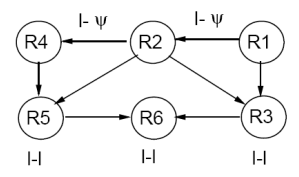
\includegraphics[width=0.7\linewidth]{images/1_1}
	\caption{مدل‌های آرایش}
	\label{fig:11}
\end{figure}
\noindent\unskip
2- روش ساختار مجازی:
\\
روش ساختار مجازی، کل نظام آرایشی شبیه یک ساختار واحد است و کلا صلب مانند. حرکت مطلوب برای مرکز ساختار مجازی القا می‌شود. با توجه به موقعیت هر کدام از رباتها نسبت به مرکز ساختار مجازی، برای هر ربات یک مسیر حرکتی اختصاص داده می‌شود. و آن ربات وظیفه‌اش دنبال کردن آن است.
\\
3- روش رفتار مبنا 
\\
رفتار مطلبوب برای ربات از قبل مشخص است. و عملکرد نهایی هر ربات بسته به وضعیت ربات از طریق وزن گذاری روی هر کدام از رفتار پیش تعیین شده و برآیندگیری از آن بدست می‌آید.
رفتار پیش تعیین شده عبارتند از :
\\
جلوگیری از برخورد با موانع، جلوگیری از بررخورد با سایر رباتها، جست و جوی هدف و حفظ شکل.

\subsection{طرح حرکت و گریز از موانع:}
در اینجا دو سوال مهم خواهیم داشت:
\\
- چه مسیری برای رسیدن به هدف باید انتخاب شود؟
\\
- با چه سرعتی و تا چه حد نزدیک به موانع باید حرکت کنند تا رباتها با اطمینان از میان موانع عبور کنند؟
\\
طرح حرکت خود می‌تواند صریح باشد یا ضمنی.
\\
طرح حرکت صریح خود شامل سه زیر بخش است:
\\
1- طرح مسیر
\\
2- طرح زمانبندی حرکت
\\
3- کنترل ربات
\\
در طرح مسیر با استفاده از داده‌های هندسی، نقاط اولیه و نقاط انتهایی دنبال ساختن راهی برای ربات هستیم تا مسئله برخورد با موانع و رسیدن به هدف بدون در نظر گرفتن سینماتیک و دینامیک طرح ریزی شود.
\\
در طرح زمانبدی حرکت با توجه به مسیرهای تولید شده در مرحله 1. هدف پیدا کردن پارامترهای زمانی زیر نظر قیود مطمئن برای منحنی‌های تولید شده است.
در انتها یک برنامه کنترلی می‌نویسیم برای تعقیب مسیرهای مطلوب.
تا زمانی که حرکت رخ ندهد، مسیر حرکت و ورودی عملگرها به صورت صریح محاسبه نخواهد شد. در حرکت ضمنی چگونگی تاثیر ربات با محیط خود تعامل با اطلاعات سنسوری و در نتیجه رفتار دینامیکی مطلوب برای ربات مشخص است. حرکت ضمنی 
\lr{Real time}
است. روش میدان پتانسیل در این دسته از روشهای طرح حرکت است.
\subsection{مروری بر پژوهش‌های پیشین:}
روش رفتار - مبنا:
یک روش کنترلی آرایش غیرمتمرکز حساب می‌شود. چون برای طراحی استراتژِی‌های کنترلی برای رسیدن به چند هدف رقابتی قابل استفاده است. در نتیجه روشی ایده آل برای تعدادی زیادی از رباتهاست.
محدودیت این روش: آنالیز ریاضی این رفتار است.
در این روش دینامیک ربات را می‌توان به عنوان ذره در نظر گرفت که در کاربردهای عملی خطای کمتری دارد.
\\
رهبر - پیرو:
مزیت این روش سادگی برای درک و کارایی در پیاده سازی است.
معایب : موقعیت راهنما در هر لحظه باید به سایر رباتها اطلاع داده شود. و پیچیدگی حذف اغتشاش داریم. یک روشی می‌توان گفت این روش کنترل متمرکز است.
\\
روش ساختار - مجازی:
ساختار آرایش به راحتی قابل توصیف است. روش کنترل متمرکز است. عیب این روش این است که تحلیل پایداری نسبت به لیدر - پیرو سخت تر است.
\\
هدف پایان نامه:
\\
ایجاد آرایش بهینه برای مجموعه‌ای از رباتهای همکار از لحاظ انرژِی برای جابجایی جسم در طی مسیری مشخص. دو روش کنترل لیدر - پیرو و ساختار مجازی برای کنترل چیدمان است. بعد این دو روش را مقایسه می‌کنیم. و هدف دیگر کنترل آرایش رباتها در فضایی با موانع طبیعی است و طرح روشی کار آمد جهت عبور گروه آرایش یافته رباتها که از میان موانع عبور کنند و به هدف مورد نظر برسند.


\section{فصل 2 
	\\
کنترل تعقیب مسیر مطلوب ربات دو چرخ محرک}
در این فصل هدف طراحی یک سیستم کنترلی برای تعقیب مسیر مطلوب برای یک ربات متحرک دو چرخ است.
این هدف با روش خطی سازی فیدبک، و ایجاد گشتاورهای مناسب به ربات جهت تعقیب مسیر مرجع امکانپذیر است. اول باید مدل دینامیکی سیستم را استخراج کنیم سپس طراجی کنترلر مطلوب بر اساس این مدل انجام می‌شود. در مرحله آخر هم تحلیل خطا و پایداری سیستم نشان دهنده کارا بودن سیستم کنترلی است.
\subsection{مدل سازی ربات}
\subsubsection{مدل سازی سینماتیکی:}
یک ربات دو چرخ محرک با یک چرخ هرزگرد برای پایداری ربات داریم. موقعیت ربات در سیستم
\lr{XY}
به وسیله بردار
\begin{equation*}
	{q}_{c} = [{x}_{c}  {y}_{c}  {\phi}]^T
\end{equation*}
مشخص می‌شود. با فرض عدم لغزش جانبی ربات تنها می‌تواند در جهت عمود بر محور رابط دو چرخ حرکت کند و این بیان کننده قید غیر هولونومیک حاکم بر سیستم است.
اگر دستگاه مختصات متصل به نقطه‌ی
\lr{${P}_{c}$}
در 
\lr{$P$}
باشد، آنگاه بردار 
$
	{q} = [{x}\space{y}\space{\phi}]^T
$
بیان کننده مختصات نقطه 
\lr{$P$}
و راستای بدنه متحرک می‌باشد.
مسئله‌ای که است بردن مبدا مختصات از نقطه 
\lr{${P}_{c}$}
به نقطه
\lr{$P$}
است. قید غیر هولونومیک تغییر پیدا می‌کند و نقطه
\lr{$P$}
در راستای محور چرخ مولفه سرعتی ندارد و  عدم لغزش چرخها در راستای جانبی.
در نهایت با نوشتن معادلات 1 تا 5 در این فصل به بردار سرعت نقطه‌ی برای نقطه 
\lr{${P}_{c}$}
خواهیم رسید.
دیگر قیدی که خواهیم داشت عدم لغزش چرخ‌های حرکت است. برای بیان غلتش خالص چرخها سرعت هر چرخ با سرعت بدنه متحرک در نقطه تماس چرخ با هم برابرند.
معادله شماره 6 برای سرعت چرخها تعریف می‌شود و در نهایت معادله شماره 5 به فرم ماتریسی نوشته شده است تا یک ماتریس رنک کامل تشکیل شود و فضای تهی اون ماتریس افراز شود.
\begin{figure}[h]
	\centering
	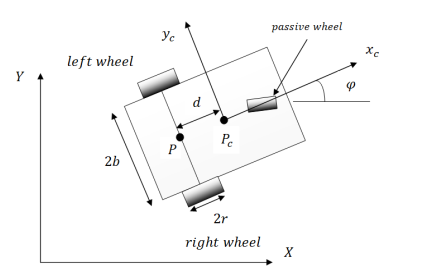
\includegraphics[width=0.7\linewidth]{images/1}
	\caption{ربات با دو چرخ محرک }
	\label{fig:1}
\end{figure}
\noindent\unskip

\subsubsection{مدل سازی دینامیکی:}
برای بدست آوردن دینامیک ربات دو حالت کلی وجود دارد یک روش معادلات نیوتن - اولر و روش دیگر معادلات لاگرانژ است.
در روش اول بر اساس نیروها و گشتاورهای وارد بر مفاصل، که معادلات حرکت سیستم بدست می‌آید.
اما این روش توی حالتی که تعداد مفاصل زیاد است خوب نیست.
روش دوم معادلات دینامیک لاگرانژ بر اساس معادلات انرژی سیستم است. در پایان نامه از روش دوم استفاده کرده است.
در معادلات لاگرانژ به انرژی جنبشی و همچنین انرژی پتانسیل نیاز داریم ولی با صفحه‌ای در نظر گرفتن حرکت بدنه محرک انرژی پتانسیل تغییر پیدا نمی‌کند با توجه به معادله 11 در نهایت معادله 12 که معادله دینامیکی ربات است را خواهیم داشت. معادله شماره 10 معادله ربات متحرک بود با جایگزین کردن معادله 10 در معادله 12 و حذف ماتریس قیدی معادله 13 بدست می‌آید. معادله 13 معادله لاگرانژ نهایی است.

\subsection{طراحی کنترلر:}
تا اینجا دو معادله اساسی داریم که یکی معدله شماره 10 است که حاصل سینماتیک ربات می‌باشد و دیگری معادله شماره 13 است که معادله نهایی بدست آمده از لاگرانژ است. معاله شماره 10 معادله سینماتیکی و معادله شماره 13 معادله دینامیکی است.
هدف از طراحی کنترلر، کنترل تعقیب مسیر مطلوب ربات رو چرخ محرک است.
برای این تعقیب مسیر میزان گشتاور اعمالی به ربات را برای طراحی مسیر خاص استفاده می‌کنیم.
معادله 14 دستور کنترلی است که پیشنهاد شده است و خطا داخل معادله 14 را اختلاف مقادیر مطلوب و واقعی متغیرهای سیستم تعریف می‌کنیم.
چون به دوبار مشتق از موقعیت در معادله 14 نیاز داریم، معادله مربوط به کنترلر پس بار دیگر از معادله 10 مشتق می‌گیریم و در معادله 14 قرار می‌دهیم. معادله 16 حاصل میشع که در واقع داره فقط گشتاور رو حساب میکنه بر اساس تغییر ات موقعیت و سرعت بر حسب زمان. حالا این معادله کنترلی و گشتاور بدست آمده را به معادله 13 که دینامیک سیستم می‌دهیم. و در نهایت معادله 17 تغییرات بردار سرعت یا بع عبارتی شتاب بدست می‌آید که با استفاده از معادله 5 و 6 می‌توان معادله 18 را برای آپدیت کردن متغیرهای مختصات سیستم و تغییراتش در زمان را در نقطه‌ی 
\lr{${P}_{c}$}
بدست آورد.
\begin{figure}[h]
	\centering
	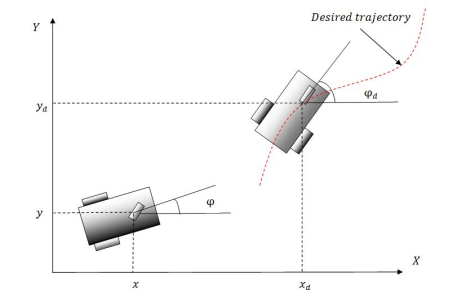
\includegraphics[width=0.7\linewidth]{images/2}
	\caption{ربات در حال تغییر مسیر، مقادیر مطلوب و واقعی سیستم}
	\label{fig:2}
\end{figure}
\noindent\unskip

\subsection{تحلیل خطا و پایداری سیستم:}
معادله 14 را با معادله 12 برابر قرار می‌دهیم و یک معادله‌ی خطا، معادله 19 بدست می‌آید. معادله خطا باید حل شود و از حل آن میفهمیم جهت پایدار شدن سیستم نحوه انتخاب ضرائب کنترلی باید بر پایه ماتریس‌های مثبت معین باشد. با این ماتریس‌ها و مفهوم پایداری همگرایی خطا به سمت صفر بدست می‌آید.
طبق گفته نویسنده تحلیل پایداری سیستم داده شده با کاندید لیاپانوف یکم سنگین است و فرایند سیستماتیکی جهت پیدا کردن چنین تابعی وجود ندارد.
اما برای اون کنترلر گفته شده در بخش قبل برای تعقیب مسیر مطلوب یک تابع کاندید لیاپانوف در فضای خطا تعریف می‌کنیم که 
\lr{quadratic}
است. از معادله 20 تا معادله 24 به این پرداخته می‌شود که تابع لیاپانوف مثبت باشد و مشتق آن منفی نیمه معین باشد و شرایط سیلوستر ارضا شود. در نتیجه سیستم پایدار مجانبی است.
!!! آنجایی که گفته شد برای سیستم لیاپانوف نداریم اما برای کنترلر کاندید هست رو خوب متوجه نشدم!!!

\subsection{خلاصه فصل:}
در این فصل ابتدا سینماتیک گفته شد و به معادله مهم شماره 10 اشاره شده که معادله سینماتیکی ربات بود. معادله شماره 10 معادله‌ای است که از قید لغزش چرخهای ربات بدست آمده است. سپس با استفاده از روش لاگرانژ معادله دینامیکی نوشته شده است که معادله شماره 13 معادله دینامیکی ربات می‌باشد. معادله شماره 14، معادله کنترلی است که پیشنهاد شده است و از ترکیب این معادله با معادله شماره 10، معادله شماره 16 را خواهیم داشت که میزان گشتاور را کنترل می‌کند و در نهایت در معادله شماره 18 هم نشان دهنده آپدیت شدن حالتهای سیستم می‌باشد. و در آخر برای معادله خطا ناشی از برابر قرار دادن معادله 12 و 14 ، یک لیاپانوف معرفی کردیم و پایداری را بررسی کردیم.

\section{فصل سوم 
	\\
	کنترل آرایش رباتهای متحرک همکار جهت جابجایی جسم:
	}
هدف از این فصل ایجاد یک الگوریتم کنترلی برای حفظ آرایش گروه است در برابر اغتشاشات. اول روش لیدر - پیرو چک می‌شود و بعد نشان داده می‌شود که این روشهای مرسوم تعقیب مسیر برای حفظ آرایش گروه در برابر اغتشاش کافی نیستند و در آخر یک الگوریتم پیشنهادی جدید به روش ساختار مجازی اضافه می‌کنیم تا در مقابل اغتشاش مقاوم بشه آرایش.
یکی از مسائل مهم محل قرارگیری هر ربات نسبت به مرکز دستگاه مختصات متصل به جسم می‌تواند از پیش تعیین شده باشد.
پس یکی از چالشها محل گیرش و نحوه‌ی آرایش رباتهاست.
هدف این پایان نامه ایجاد آرایش بهینه برای مجموعه رباتها در حین حمل بار است.

\begin{figure}[h]
	\centering
	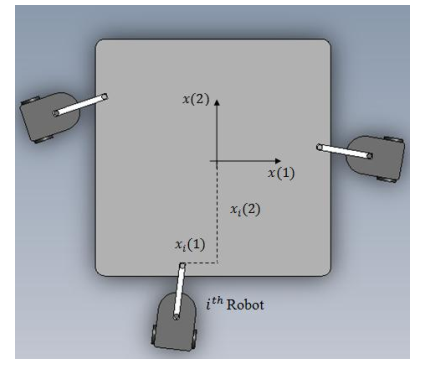
\includegraphics[width=0.7\linewidth]{images/3}
	\caption{سه ربات متحرک به همراه جسم مورد جابجایی}
	\label{fig:3}
\end{figure}
\noindent\unskip
از نقطه نظر فضای عملکرد دو دسته کلی داریم:
دسته‌ای که در آنها مجموعه‌‌هایی بیرون از خود سیستم مکانیابی می‌شوند و در واقع یک سیستم مختصات جهانی داریم.
دسته دیگر موقعیت یابی محلی یعنی نسبت به یکدیگر است.
اکثر طراحی‌های کنترلی برای سیستم محلی انجام می‌شود در این پژوهش هم سیستم محلی در نظر گرفته شده است.
\subsection{کنترل آرایش: روش لیدر - پیرو:}
هدف حفظ فاصله نسبی بین رباتهاست. دو نوع طرح کنترلی داریم. در طرح فاصله - زاویه هر ربات پیرو قادر به تشخیص فاصله و زاویه نسبت به ربات رهبر گروه است. این روش موقعی خوب است که هر ربات از یک ربات لیدر پیروی کند.
طرح دوم فاصله - فاصله است در این طرح هر ربات پیرو برای حفظ آرایش در گروه فاصله نسبی خود را نسبت با دو ربات دیگر اندازه‌گیری می‌کند.
در این پایان نامه از روش اول استفاده شده است.
با پارامترهای 
\lr{$ L, \theta$}
ربات پیرو می‌تواند فاصله نسبی خود را با ربات لیدر ایجاد کند.
هدف از روش لیدر - پیرو این است که رباتها یک جسمی را در طی مسیری جابجا کنند. پس دوتا مسیر می‌نویسیم یکی برای لیدر و دیگری برای پیرو. معادلات 2 و 3 اشاره به مسیر لیدر دارند. جهت اجرای وظیفه جابجایی جسم برای سایر رباتها که پیرو ربات راهنما هستند باید مسیری مشخص کنیم که معادلات 4و5 به این امر پرداخته‌اند.
برای اجرای وظیفه حمل جسم پارامترهای آرایش برای رباتهای پیرو با توجه به سه نکته طراحی می‌شود: موقعیت گیرش ربات پیرو، موقعیت مرکز دستگاه مختصات متصل به جسم، فاصله رباتها نسبت به راهنمای گروه. معادله 6 بدست خواهد آمد.
حال با توجه به این معادلات مسیر مطلوب تعیین شده است.
در مرحله جدید باید یک کنترلر برای هر ربات جهت تعقیب مسیر مرجع برای ایجاد آرایش تولید شود.

\begin{figure}[h]
	\centering
	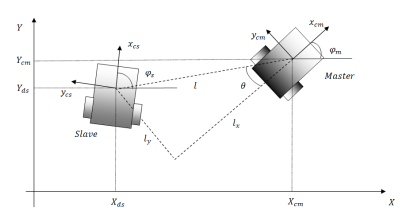
\includegraphics[width=0.7\linewidth]{images/4}
	\caption{روش فاصله -زاویه}
	\label{fig:4}
\end{figure}
\noindent\unskip

\subsubsection{شبیه سازی:}
در این بخش یک روش کنترلی را روی 3 ربات انجام داده‌‌اند برای تشکیل آرایش مثلث شکل. در دو حالت تست انجام شده است حالت بدون اغتشاش و حالت با اغتشاش.
ابتدا یک مسیر مرجع با معادله شماره 8 درست شده است.
در معادله شماره 8، 
\lr{${y}_{d}$}
یک معادله درجه پنج است برای حرکت راستای جسم.
محل گیرش رباتها نسبت به دستگاه مختصات متصل به جسم را می‌خواهیم.
برای نشان دادن آرایش شکل گرفته یک خطای جدید به نام خطای فاصله بین رباتها تعریف می‌کنیم، که این خطا تفاوت بین فاصله واقعی و فاصله دلخواه است.
باید در شبیه سازی خطا در سه راستا و این خطای فاصله را نشان دهیم.
و همچنین نمودار های مربوط به گشتاورهای چرخ‌های هر ربات را نشان می‌دهیم.
در روش لیدر - پیرو چون از سمت پیرو به سمت لیدر هیچ سیگنالی ارسال نمی‌شود در نتیجه انتظار می‌رود که آرایش گروه در حین اغتشاش از بین برود.
مثلا روی ربات شماره 2 که پیرو است به مدت 5 ثانیه اغتشاش دادیم و تمامی نمودارهای بالا چک می‌شوند.
دیده می‌شود که آرایش مجموعه‌ای در حین اجرای وظیفه از بین می‌رود. این مساله یکی از ایرادهای این روش است جون هیچ فیدبکی از سمت پیرو به سمت لیدر نیست و سیستم در مقابل اغتشاش مقاوم نیست.
اگر بخواهیم فیدبکی از سمت پیرو به لیدر داشته باشیم در نتیجه این اغتشاش در ربات لیدر ظاهر می‌شود. (معادله شماره 4) و در نتیجه باعث ناپایداری آرایش گروه می‌شود.
هدف پروژه ایجاد یک روش جدید است که در مقابل اغتشاش قوی باشد.

\section{کنترل آرایش روش ساختار مجازی:}
\subsection{طراحی کنترلر}
جسم صلبی را در نظر می‌گیریم که نقاط متصل به این جسم فاصله نسبی مشخصی را نسبت به دستگاه متصل به بدنه جسم صلب دارا هستند. وقتی این جسم صلب در فضا حرکت کند نقاط متصل به این ساختار با حفظ فاصله نسبی خود نسبت به دستگاه متصل به بدنه در فضا جابجا می‌شوند. حالا این نقاط همون رباتها هستند. این رباتها فاصله‌ای مشخص را نبست به دستگاه متصل به جسم صلب اختیار می‌کنند. خود رباتها هم یک فاصله مشخص را نسبت به هم دارند. این رباتها با جسم صلب را، ساختار مجازی گوییم و این ساختار مجازی رو کنترل می‌کنیم.
یعنی این ساختار مجازی منطبق بر جسمی است که رباتها قصد حمل آن را دارند. پس وقتی مرکز ساختار مجازی جابجا شود با توجه به موقعیت هندسی رباتها نسبت به مرکز، برای رباتها تولید مسیر می‌شود.

\begin{figure}[h]
	\centering
	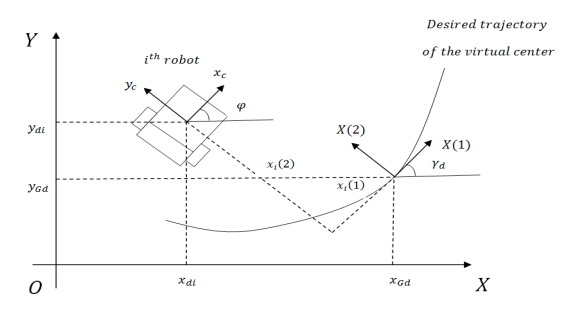
\includegraphics[width=0.7\linewidth]{images/5}
	\caption{مسیر  ساختار مجازی و نحوه قرارگیری رباتها}
	\label{fig:5}
\end{figure}
\noindent\unskip
چون ساختار مجازی قسمت از جسم است پس در این روش پارامترهای گیرش با پارامترهای آرایش جسم برابر است.
معادله 10 مسیر مطلوب هر ربات را با استفاده از مسیر مطلوب جسم بدست میارد.
اهداف کنترلی در روش ساختار مجازی عبارت است از:
1- تمام آرایش مسیر از پیش تعیین شده را تعقیب کند. یعنی هر ربات مسیری که از مرکز ساختار مجازی تولید میشه را دنبال می‌کند.
2- رباتی دچار مشکل شد هر ر بات وظیفه تعقیب مسیر مرجع و آرایش را تکمیل کند.
از اونجایی که هر ربات موقعیت هندسی مشخصی نسبت با ساختار مجازی داره پس وقتی انحرافی پیش میاد این انحراف در موقعیت مرکز ساختار مجازی است و باید یک موقعیت جدید بدست بیاریم.
معادله 11 برای بدست آوردن انحراف است.
میزان انحراف هر ربات را نسبت به یکدیگر بدست می‌یاریم و تغییرات را به مسیر ربات اضافه می‌کنیم.
بعد دوباره یک برداری از خطا درست می‌کنیم که از آنجایی که در روش ساختار مجازی صرفا مکان رباتها نسبت به یکدیگر کنترل می‌شود. پارامتر دوران صفر است. هر ربات علاوه بر فیدبک خودش یک فیدبک هم از باقی رباتها می‌گیرد.
معادلات 14 تا 16 گشتاور کنترلی مورد نیاز را تعریف می‌کنند. معادله 16 که از مشتق گیری از خطا بدست آمده است که نیروی فنر دمپر مجازی را مدل می‌کند که باعث اتصال رباتها با یکدیگر می‌شود.

\begin{figure}[h]
	\centering
	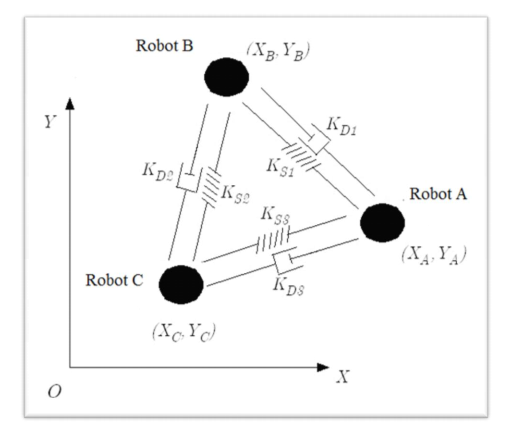
\includegraphics[width=0.7\linewidth]{images/6}
	\caption{فنر دمپر مجازی}
	\label{fig:6}
\end{figure}
\noindent\unskip

\subsection{تحلیل خطا}
با قرار دادن ورودی کنترلی در سیستم دینامیکی ربات معادله‌ی 17 بدست میاد بعد یک ترم برای خطا تشکیل می‌دهیم در معادله 18 تا برای این ترم یک تابع کاندید لیاپانوف تعریف کنیم و با اینکه این تابع لیاپانوف شرایط سیلوستر را داشته باشد نشان داده می‌شود که خطای سیستم مورد نظر به صفر همگرا می‌شود.

نتیجه گیری:
در کنترل آرایش با روش لیدر - پیرو، حذف افتشاشات در سیستم با دشواری زیادی همراه خواهد بود. و در ضمن اینکه حفظ آرایش با مشکل کواجه خواهد شد. در روش ساختار مجازی با اعمال کنترلر آرایش مجموعه رباتها در حین اغتشاش به خوبی برقرار خواهد بود. روش ساختار مجازی از لحاظ حرکت برای رباتها و چه از لحاظ کنترل روشی مناسبتر است جهت کنترل آرایش مجموعه رباتها برای حمل جسم.
\section{گریز از موانع و کنترل آرایش رباتهای متحرک همکار}
در این فصل سعی در ایجاد راهکاری جهت عبور مجموعه‌ی رباتها در حین جابجایی جسم از میان موانع هستیم.
در این فصل با توجه به میدان پتانسیل مصنوعی و معرفی روش پسخوراند آرایش و در نظر گرفتن روش ساختار مجازی وظیفه‌ی جابجایی جسم انجام می‌شود.

\subsection{روش میدان پتانسیل مصنوعی:}
ایده اصلی روش میدان پتانسیل مصنوعی این است که هدف مثل یک چاه است و کمینه میدان پتانسیل را دارد و نیروی جاذبه ایجاد می‌کند و مانع‌ها تپه‌های بلند میدان هستند که بیشینه میدان را دارند و نیروی دافعه تولید می‌کنند.
در آخر یک میدان کل داریم که برایند نیروی جاذبه و دافعه است.
میدان پتانسیل جاذبه:
\\
تمام نقاط فضای کاری یک جریان گرادیان منفی جهتی به سمت هدف دارند.
معادله شماره 1 معمول ترین گرادیان پتانسیل جاذبه است.
این معادله تابعی از فاصله بین ربات تا هدف است.
میدان پتانسیل دافعه:
\\
پتانسیل دافعه مانع به صورت یک دیسک مدور مدل می‌شود و تمام خصوصیات یک مانع را می‌تواند داشته باشد.
این پتانسیل دافعه یک تابع از فاصله بین ربات تا مانع است و محدوده مانع در میدان پتانسیل است.
این تابع مشکل کمینه محلی را دارد یعنی وقتی هدف بیش از حد نزدیک به مانع باشد منجر به کمینی محلی می‌شود که معادله 2 به معادله شماره 3 تغییر پیدا می‌کند. ترمی که اضافه می‌شود کوتاه ترین فاصله بین ربات تا هدف است.
و این اطمینان را ایجاد می‌کند که تابع پتانسیل کل در کمینه قرار گیرد. اگر و تنها اگر ربات به هدف دست پیدا کند یعنی این فاصله صفر باشد.
\\
\begin{figure}[h]
	\centering
	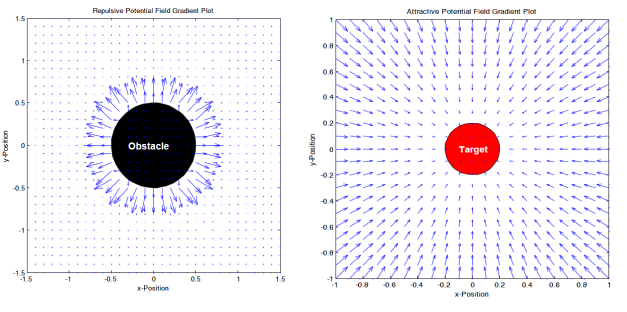
\includegraphics[width=0.7\linewidth]{images/7}
	\caption{میدان جاذبه و میدان دافعه}
	\label{fig:7}
\end{figure}
\noindent\unskip

میدان پتانسیل کل:
\\
با برآیند دو میدان جاذبه و دافعه میدانی بدست خواهد آمد که شکل کلی آن در مواقعی غیرقابل پیش بینی است. پس نتیجه این مشکل به وجود آمدن مشکل کمینه محلی است که باعث به دام انداختن ربات خواهد شد و ربات دیگه حرکت نمی‌کند.
\\
\begin{figure}[h]
	\centering
	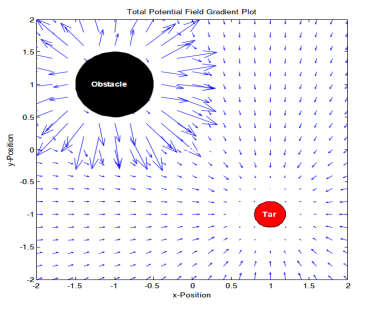
\includegraphics[width=0.7\linewidth]{images/8}
	\caption{تابع پتانسیل کل}
	\label{fig:8}
\end{figure}
\noindent\unskip

عیوب این روش:
\\
اگر دو مانع خیلی نزدیک هم قرار بگیرند و میدان جاذبه به اندازه کافی قوی نباشد، ربات توانایی گذر از میان موانع را ندارد.
ایراد دیگه این روش بهینه نبودن مسیر آن است. با توجه به اینکه مسیر حرکت صریح نیست مسیری که از گرادیان میدان ایجاد می‌شود بهینه نخواهد بود.
رباتها در حین عبور از میان موانع با سرعت زیاد دچار نوسان می‌شوند که شبیه اغتشاش هست ولی توی سرعت پایین این نوسانات رو نداریم.
خب مسئله این است که این الگوریتم الان برای یک ربات طرح حرکت ایجاد می‌کند. پس باید یک تغییراتی داد تا برای چند ربات با حمل جسم این الگوریتم کار کند.

\subsection{گریز از موانع و کنترل آرایش برای مجموعه رباتها:}
در این پروژه ساختار مجازی به جای لیدر - پیرو انتخاب شده است. مرکز ساختار مجازی با استفاده از پارامترهای آرایش برای سایر رباتها، مسیر مطلوب ایجاد می‌کند. پس با استفاده از موقعیت مرکز ساختار مجازی و قرار دادن آن می‌توان گروه آرایش یافته را از میان موانع عبور داد.
معادلات جدید شماره 5 تولید می‌شوند که در آن به جای موقعیت ربات، موقعیت ساختار مجازی را قرار می‌دهیم. در نهایت گروه آرایش یافته را از میان موانع عبور می‌دهیم.
در این روش باید محدوده موثر مانع را بیشتر دقت کنیم. برای تعیین این پارامتر فرض می‌کنیم که گروه آرایش یافته رباتها به همراه جسم مورد جابجایی در دایره‌ای به شعاع 
\lr{R}
قرار می‌گیرند. این انتخاب شعاع دایره به جسم مورد جابجایی و نحوه آرایش ربات بستگی دارد.

\begin{figure}[h]
	\centering
	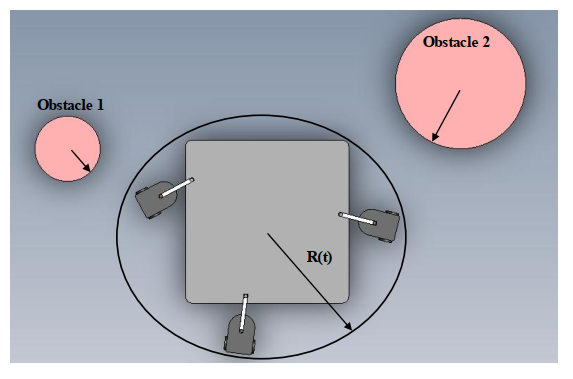
\includegraphics[width=0.7\linewidth]{images/9}
	\caption{دایره آرایش و موانع}
	\label{fig:9}
\end{figure}
\noindent\unskip
\\
برای تمام نقاط در داخل محیط کاری رباتها اطلاعات گرادیان موجود است و با استفاده از اطلاعات گرادیان میدان پتانسیل ورودی لازم جهت حرکت رباتها تعیین می‌شود. وقتی که رباتها در پایین ترین نقطه میدان که هدف در آنجا است قرار بگیرند مقادیر گرادیان صفر میشه و ربات متوقف می‌شود.
حالا مشکلی که داشتیم این بود که قوام آرایش را داشته باشیم. اگر یکی از  رباتهای گروه یا تمام گروه آرایش یافته دچار اشکال شود پسخوراندی از گروه رباتها به مرکز ساختار مجازی ارسال نمی‌شود پس این فیدبک رو اضافه می‌کنیم. پس فرض می‌کنیم هرگاه رباتها آرایش خود را از دست دادند مرکز ساختار مجازی از سرعت خود بکاهد یا متوقف شود. از طرفی دیگر می‌خواهیم وقتی رباتها در آرایش قرار گرفتند، محموعه با سرعت مطلوب به سمت هدف برود.
یک تابع پسخوراند آرایش تعریف می‌کنیم، معادله 11 که تابعی از اختلاف ماتریس موقعیت مطلوب گروه و موقعیت گروه ربات است. پس در نهایت سرعت مرکز ساختار مجازی  یک فیدبکی از آرایش گروه می‌گیرد.

\subsection{شبیه سازی و ارائه نتایج:}
یک موقعیت اولیه برای مرکز ساختار مجازی در نظر می‌گیریم و راستا ساختار صفر است.
مانع‌ها را می‌گذاریم و مختصات موانع و شعاعشون رو مقدار دهی می‌کنیم.
بعد پارامترهای کمترین فاصله موانع را تعریف می‌کنیم. در مرحله بعدی موقعیت نهایی هدف در یک مختصات خاص را تعریف می‌کنیم.
برای هر ربات هم یک شرایط اولیه موثر در نظر می‌گیریم.
دو فیدبک هم داشتیم: فیدبک متقابل و فیدبک آرایش.

\section{کنترل امپدانش چندگانه و آرایش بهینه رباتهای متحرک همکار:}

در مورد کنترل امپدانس واقعا نفهمیدم.

\subsection{آرایش بهینه مجموعه رباتهای متحرک همکار:}
در مورد بهینه سازی صحبت شده و اینکه دسته بندی بهینه سازی در 4 دسته کلی. در مورد الگوریتم‌های الهام گرفته از طبیعت و الگوریتم‌های تحلیلی و قطعی صحبت شده و اینکه مزیت و عیب این الگوریتمها گفته شد. سپس سه الگوریتم پرواز پرندگان، ژنتیک، شبیه سازی حرارتی مورد بررسی قرار گرفت.


